\begin{flushright} {\tiny {\color{gray} (tikz\_P1.tex)}} \end{flushright}
%~~~~~~~~~~~~~~~~~~~~~~~~~~~~~~~~~~~~~~~~~~~~~~~~~~~~~~~~~~~~~~~~~~~~~~~~~~~~~~~~~~~~~~~~~~~~~~~~~~

\begin{center}
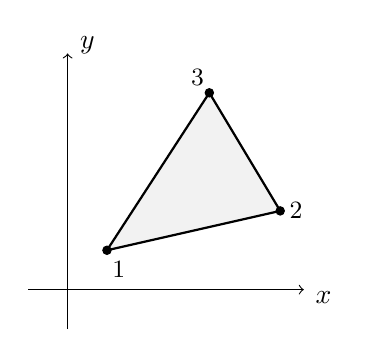
\begin{tikzpicture}
%\draw[step=0.5cm,gray,very thin] (0,0) grid (4,4); 
\draw[fill=gray!10,gray!10](1,1) (1,1)--(3.2,1.5)--(2.3,3)--cycle;
\draw[thick] (1,1)--(3.2,1.5)--(2.3,3)--cycle;
\draw [->] (0,0.5) -- (3.5,0.5);
\draw [->] (0.5,0) -- (0.5,3.5);
\node[] at (3.75,0.4) {$x$};
\node[] at (0.75,3.6) {$y$};
\draw[black,fill=black] (1,1)   circle (1.5pt);
\draw[black,fill=black] (3.2,1.5)   circle (1.5pt);
\draw[black,fill=black] (2.3,3)   circle (1.5pt);
\node[] at (1.15,0.75) {\small $1$};
\node[] at (3.4,1.5) {\small $2$};
\node[] at (2.15,3.2) {\small $3$};
\end{tikzpicture}
\end{center}


